 \chapter{Fine-tuning di LLM attraverso LoRA e ottimizzazioni}
\label{chap:descrizione-stage-2}
\section{Analisi del dominio applicativo}
Nella seconda fase del progetto si è proceduto con il \gls{fine-tuning} di un \gls{llm} attraverso \gls{lora}, e le sue ottimizzazioni, come ad esempio \textit{MoLE} e \textit{AdaMoLE}. In questo capitolo si approfondiranno inoltre gli studi effettuati sul \gls{fine-tuning} e quantizzazione, concentrandosi maggiormente sul possibile apporto valoriale che questi ultimi possono dare ad un \gls{llm} e alle sue implementazioni.
Questo poichè moltissime realtà aziendali si stanno concentrando sul \gls{fine-tuning} di modelli preaddestrati, in quanto permette di adattare un modello ad un nuovo dominio, senza doverlo addestrare da zero.
%porzione del mondo reale con cui si deve interagire
    \subsection{Analisi del tema}
    Nella seconda parte del progetto, vi è stata una maggiore attenzione posta principalmente sullo studio delle tecniche di \gls{fine-tuning} e quantizzazione, poiché rappresentano argomenti complessi e nuovi nel settore. In particolare, la lettura di diversi articoli scientifici e la realizzazione di esperimenti su \textit{Colab} sono stati fondamentali per comprendere a fondo queste tecniche. Queste attività sono state inoltre indispensabili per poter applicare in modo pratico le nozioni apprese.
    Questa fase del progetto si distingue inoltre dalla prima poiché si è focalizzata maggiormente sulla ricerca e sperimentazione di nuove metodologie rispetto all'applicazione pratica immediata. Tuttavia, sebbene il focus principale fosse la ricerca, vi è stata comunque la possibilità di applicare queste tecniche in modo pratico tramite l'utilizzo di \textit{Colab}.

    %descrive il dominio del problema da affrontare:
    %la porzione del mondo reale, rilevante per il sistema\\
    %-> Su cui si devono mantenere informazioni\\
    %-> Concuisideve interagire

    %LoRA e quantizzazione -> perchè sono utilizzati 

    \subsection{Esempi di utilizzo}
   Al giorno d'oggi, le possibili applicazioni di un \gls{llm} \textit{fine-tuned} sono molteplici e spaziano dalla generazione di codice sorgente alla traduzione di testi. Queste tipologie di utilizzo sono chiamate \textit{downstream task}, poiché sono \textit{task} eseguite dopo il preaddestramento del modello e si concentrano su argomenti specifici. Le \textit{downstream task} rappresentano quindi la motivazione principale per effettuare il \gls{fine-tuning} di un modello preaddestrato. Lo scopo di questa attività è far concentrare il modello su un particolare dominio, migliorando così le performance in quei compiti specifici rispetto a un modello preaddestrato generico.
Per quanto riguarda la quantizzazione, l'utilizzo di modelli quantizzati è oggi pressoché fondamentale. I modelli non quantizzati richiedono infatti troppa memoria e potenza di calcolo, rendendo difficile per la maggior parte delle aziende utilizzare modelli di \gls{llm} senza questa tecnica di ottimizzazione.

    %dare la possibilità all'LLM di rispondere a domande sul dominio downstram task
    % rendere disponible i modelli anche su macchine più piccole ad esempio microcontrollori
    \subsection{LoRA}
    \gls{lora} è un metodo di \gls{peft} che permette di adattare un modello preaddestrato ad un nuovo dominio, attraverso l'aggiunta di un \textit{layer}.
    Questa metodologia di \gls{fine-tuning} viene introdotta da J. Edward Hu et al.\cite{article:Hu2021LoRALA} e consiste nel congelare i pesi del modello preaddestrato e inserire delle \textit{trainable rank decomposition matrices} come un \textit{layer} aggiuntivo.
    Queste matrici permettono di diminuire notevolmente il numero di parametri da addestrare, rendendo il \gls{fine-tuning} più veloce e meno costoso.
    La costruzione delle \textit{trainable rank decomposition matrices} A e B avviene attraverso la decomposizione di della matrice di pesi W in due matrici di rango ridotto.
    Supponiamo di avere una matrice preaddestrata $W_0 \in \mathbb{R}^d^\times^k$, e voler aggiungere un \textit{layer} $\Delta W$ per il fine tuning, allora possiamo scrivere:\newline 
    \centerline{$ W_0 + \Delta W = W_0 + BA$ ,}
    \newline 
    dove $B \in \mathbb{R}^d^\times^r$ e $A \in \mathbb{R}^r^\times^k$ con rank $r \ll min(d, k)$. 
    In questo modo è possibile addestrare solamente un insieme più piccolo di parametri i quali, moltiplicati tra loro, si avvicinano alla matrice di pesi più ampia nel modello pre-addestrato.
    \begin{figure}[htp]
        \centering
        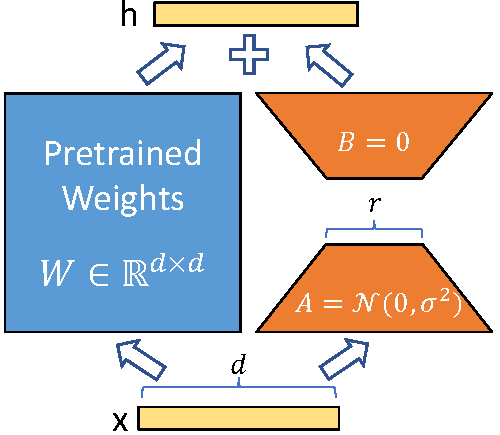
\includegraphics[alt={Testo alternativo dell'immagine}, width=0.5\columnwidth]{img/figure1.pdf}
        \caption{LoRA matrices}
        \label{fig:entanglement}
    \end{figure}
    \newline
    $A$ e $B$ vengono rispettivamente inizializzati attraverso la funzione Gaussiana e 0, quindi il valore all'inizio dell'addestramento della matrice $W$ è 0. Attraverso le iterazioni, i parametri verranno modificati e si otterrà un \textit{layer} LoRA che permetterà al modello di avere capacità più specifiche.
    Notiamo quindi che la quantità di dati da aggiornare è nettamente minore, si dovrà infatti addestrare solo $A$ e $B$. In particolare, l'utilizzo della VRAM diminuisce di 2/3 se  $r \ll d_m_o_d_e_l$.
    L'utilizzo di \gls{lora} porta ad alcuni vantaggi oltre al risparmio di memoria, l'addestramento infatti risulta più efficiente ed inoltre è possibile creare tanti \textit{layers} \gls{lora} in modo da poterli interscambiare in base alle esigenze.
    %cos'è, come funziona e spiegazione matematica con qualche immagine delle matrici
    \subsubsection{Future applicazioni} 
    Le future applicazioni che durante questo stage sono state prese in considerazione con il tutor aziendale Gregorio Piccoli e sono legate soprattutto alla possibilità di utilizzare modelli 
    \textit{fine-tuned} per rispondere a domande sul dominio \textit{downstream task}, come ad esempio la generazione di codice sorgente.
    Un ulteriore utilizzo potrebbe essere legato al compilatore dei linguaggi di programmazione, in modo tale da avere un feedback logico del programma oltre che sintattico e semantico.
    Inoltre, un'altra possibile applicazione è quella di rendere disponibili i modelli attraverso la quantizzazione anche su macchine più piccole, come ad esempio microcontrollori. Questa possibilità al giorno d'oggi permetterebbe l'utilizzo 
    di \gls{llm} in dispositivi che non hanno una potenza di calcolo elevata, come ad esempio gli smartphone.

    
\section{Analisi dei requisiti}
    \subsection{Analisi preventiva dei rischi}
    Durante la fase di analisi dei rischi sono stati individuate le possibili criticità che potranno essere riscontrate.
    Si è quindi proceduto a elaborare delle possibili soluzioni per far fronte a tali rischi.
    \begin{risk}{Mancanza di risorse computazionali}
        \riskdescription{Essendo il \gls{fine-tuning} un processo molto oneroso, la quantità di risorse computazionali a disposizione potrebbe risultare quindi non sufficiente per addestrare modelli molto grandi}
        \risksolution{utilizzo di Colab e coinvolgimento del responabile aziendale}
        \label{risk:data-absence} 
    \end{risk}

    \subsection{Requisiti e obiettivi}

    \begin{center}
        \rowcolors{1}{}{tableGray}
        \begin{longtable}{|p{2.25cm}|p{7.75cm}|p{2.25cm}|}
        \hline
        \multicolumn{1}{|c|}{\textbf{Obiettivo}} & \multicolumn{1}{c|}{\textbf{Descrizione}}\\ 
        \hline 
        \endfirsthead
        \multicolumn{3}{c}%
        {{\bfseries \tablename\ \thetable{} -- Continuo della tabella}}\\
        \hline
        \multicolumn{1}{|c|}{\textbf{Obiettivo}} & \multicolumn{1}{c|}{Descrizione}\\ \hline 
        \endhead
        \hline
        \multicolumn{3}{|r|}{{Continua nella prossima pagina...}}\\
        \hline
        \endfoot
        \endlastfoot 
        OB 4 & Realizzazione di test con LLM fine-tuned attraverso \gls{lora}. \\
        \hline
        DE 1 & Quantizzazione di LLM. \\
        \hiderowcolors
        \caption{Requisiti secondo macroperiodo.}
        \label{tab:requisiti_obbiettivi}
        \end{longtable}
    \end{center}



\section{Sviluppo del prodotto}
Lo sviluppo del prodotto durante il secondo macroperiodo non è stato immediato come è successo durante prima  parte, questo poichè è stato necessario studiare in modo approfondito gli argomenti che sarebbero stati trattati successivamente. Dopo lo studio della teorica legata al \gls{fine-tuning} e  quantizzazione, è stato necessario studiare anche le tecniche di applicazione, ciò è avvenuto simultanemanete alla loro implementazione, vi è stato quindi un'applicazione della metodologia di apprendimento \textit{learing by doing}.
Inoltre, è stato necessario preparare un dataset attraverso il quale effettuare il \gls{fine-tuning}.
%studio iniziale di LoRA e quantizzazione perchè sono argomenti complessi e nuovi
%trovare dataset con il quale fare fine-tuning
    \subsection{\textit{Fine-tuning attraverso Pytorch}}
     Il \gls{fine-tuning} è un processo costoso, per questo motivo si è scelto di eseguirlo su \textit{Colab}, utilizzando un account Pro, il quale offre 100 unità di calcolo. Di seguito viene spiegato il processo di \gls{fine-tuning} attraverso il codice utilizzato.
     È possibile in figura 4.2 trovare il codice relativo alla configurazione di \gls{lora}.
    %CODICE LoRA
    \begin{figure}[!h]
        \centering        
        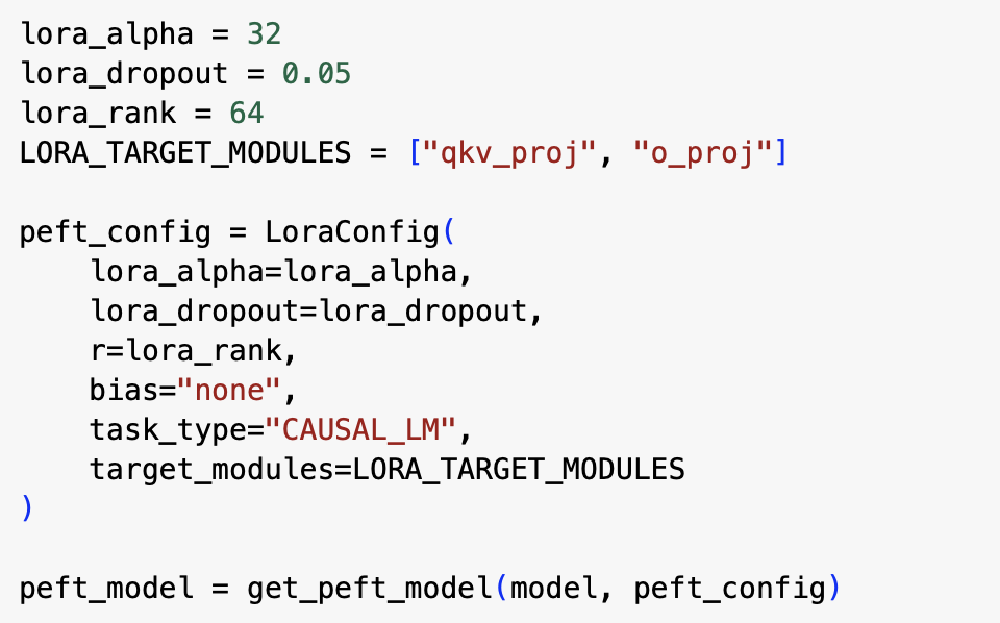
\includegraphics[width=12cm]{img/codiceLoRA.pdf}
        \caption{Configurazione parametri \gls{lora}}
    \end{figure}\newline
\begin{itemize}
    \item \textbf{lora\_alpha} determina l'entità della riduzione del rango durante il processo di approssimazione \textit{Low Rank}. Un valore più alto di \textit{lora\_alpha} comporta una riduzione più aggressiva del rango, risultando in una maggiore compressione delle matrici dei pesi e in un modello più efficiente in termini di parametri. Al contrario, un valore inferiore di \textit{lora\_alpha} comporta una riduzione meno aggressiva del rango, preservando più parametri del modello originale.
    \item \textbf{lora\_rank} esprime invece il rango della matrice decomposta. Un rango maggiore implica un maggiore utilizzo di memoria, mentre un rango minore riduce l'impatto sulla memoria ma comporta una perdita di informazioni. Diventa quindi cruciale trovare il rango più adeguato per bilanciare l'efficienza della memoria e la conservazione delle informazioni.
    \item \textbf{lora\_dropout} è la probabilità di eliminare elementi dalle matrici $A $ e $B$ per evitare \textit{overfitting}.
    \item \textbf{LORA\_TARGET\_MODULES} sono i moduli dei layer ai quali verrà applicato \gls{lora}. In questo caso, \gls{lora} è stato applicato ai moduli \textit{qkv\_proj}, \textit{o\_proj} presenti come visibile in figura 4.4 nella \textit{self attention} come suggerito da et al. \cite{article:Hu2021LoRALA} .
    È importante notare che i moduli in questione potrebbero cambiare in base al modello e alla sua architettura interna.
    \end{itemize}

In figura 4.3 è possibile quindi visualizzare l'architettura di \textit{Phi3-mini}, uno dei modelli al quale è stato applicato il \gls{fine-tuning}, \textit{Phi3-mini} è un \textit{state-of-the-art open model} , il quale si basa sull'architettura \textit{Transformer} ed è stato pre-addestrato sia con dati pubblici ma anche sintetici. 
    \begin{figure}[!h]
        \centering        
        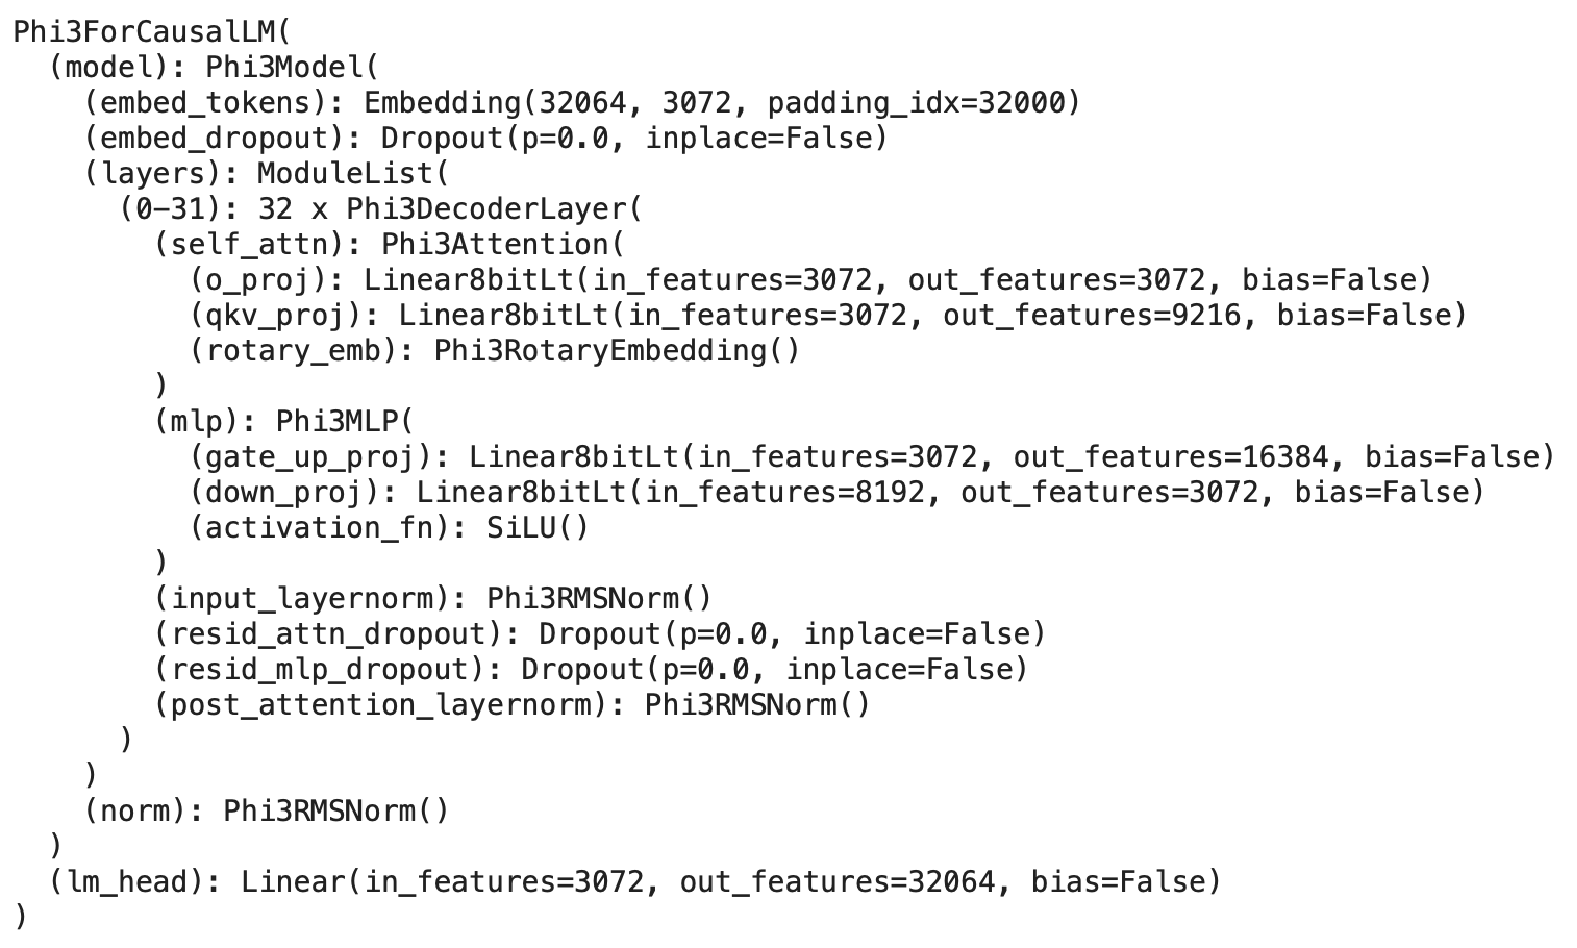
\includegraphics[width=14.5cm]{img/Phi3.pdf}
        \caption{Architettura di \textit{Phi3-mini}}
    \end{figure}

    \begin{figure}[!h]
        \centering        
        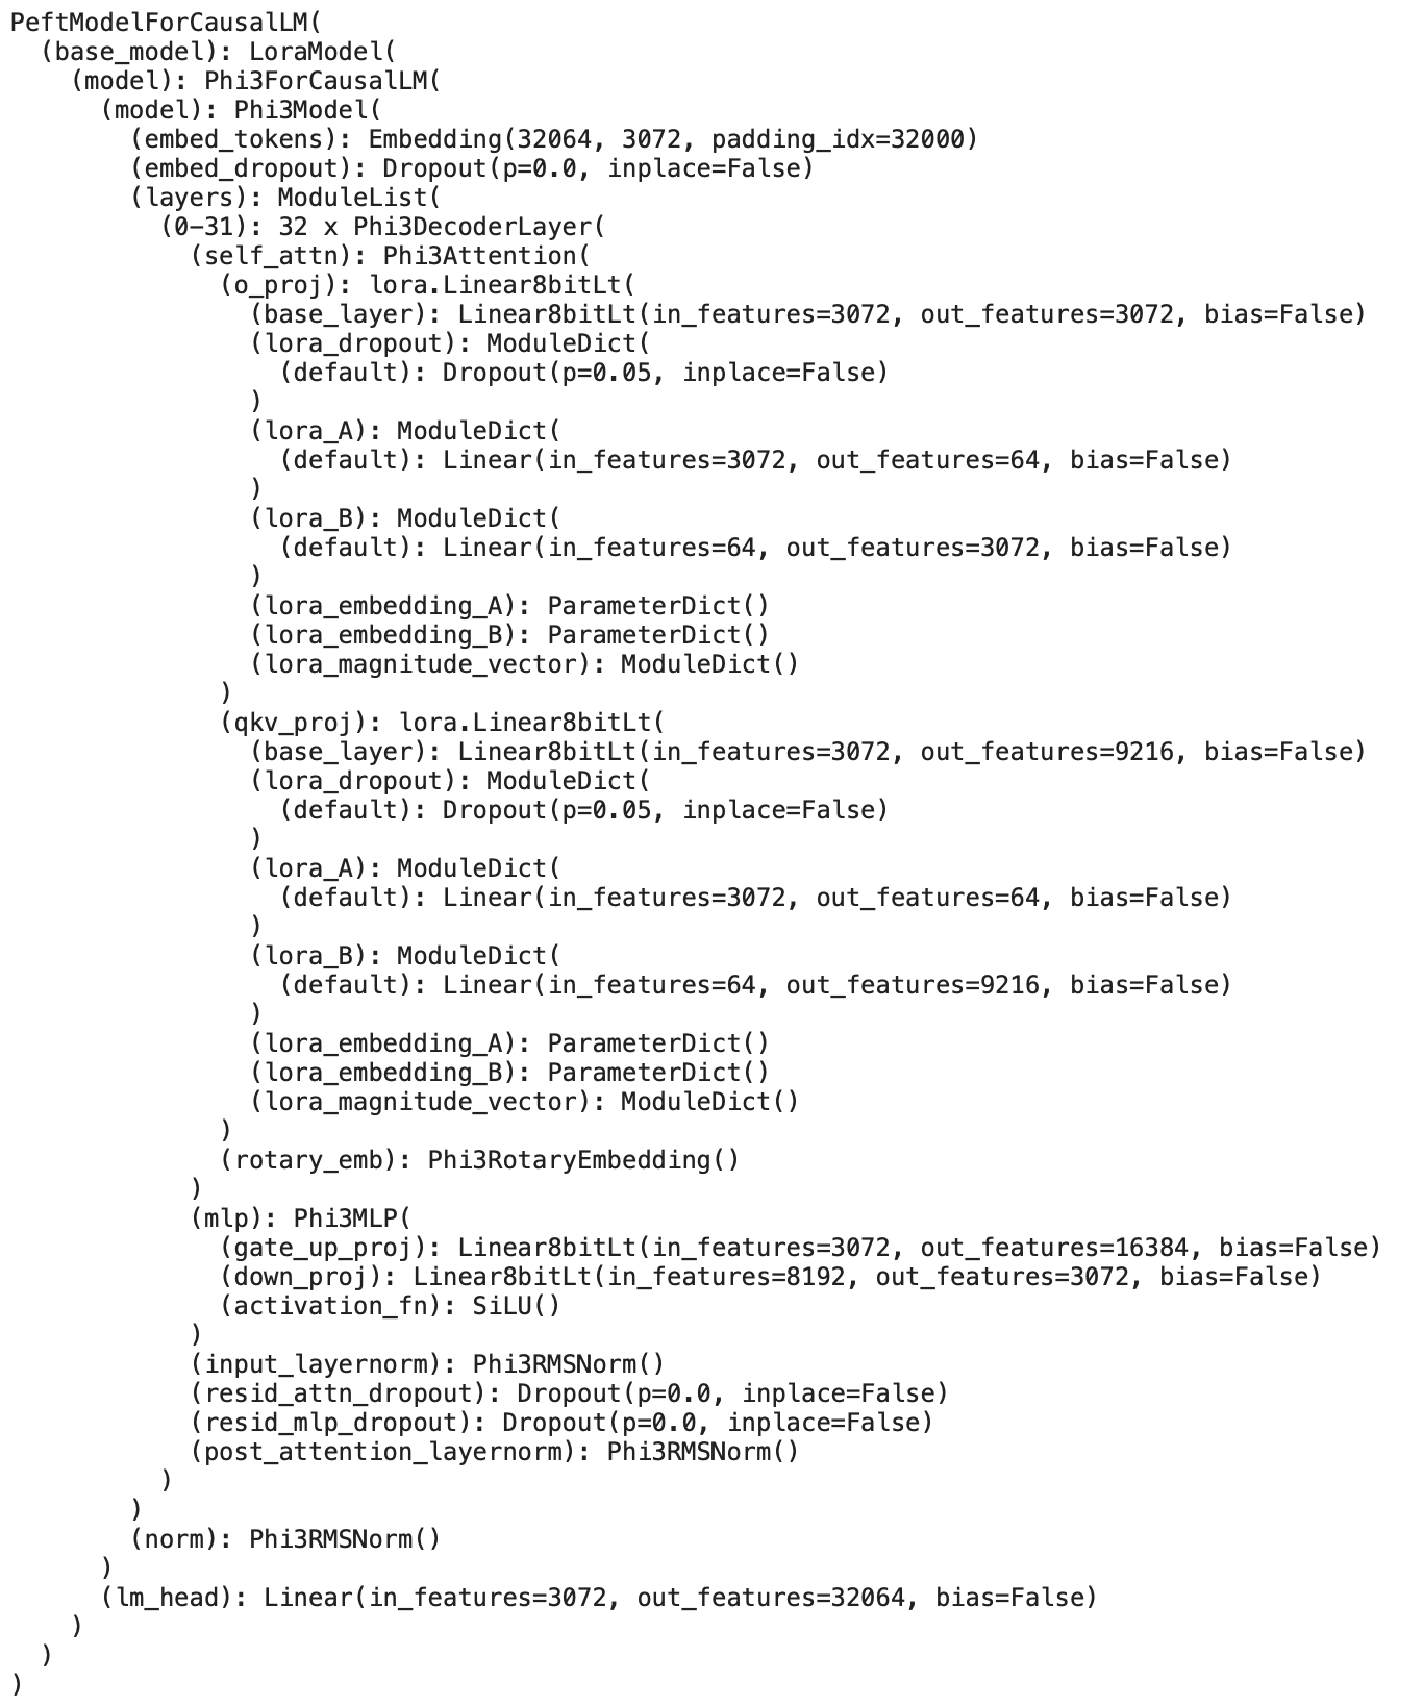
\includegraphics[width=14.5cm]{img/LoRA.pdf}
        \caption{Applicazione \gls{lora} a \textit{Phi3-mini}}
    \end{figure}\newpage
    
    Nella figura 4.4 possiamo notare il risultato ottenuto dall'applicazione di \gls{lora}. 
    
    %scrivi che si vede che lora è applicato ed infatti si vede che ci sono i layer sui moduli e sono di grandezza 64
    
    Successivamente, è stato necessario trovare un \textit{dataset} appropriato per il \gls{fine-tuning}. È stato scelto "\textit{Vezora/Tested-22k-Python-Alpaca}", che contiene ben 22.600 esempi di codice testato. Il dataset, suddiviso in istruzioni, input e output, è stato formattato correttamente come mostrato in figura 4.5 per seguire il \textit{prompt} con cui il modello di partenza è stato addestrato. Questo passaggio è cruciale poiché ogni \gls{llm} richiede un determinato \textit{prompt}. Senza il \textit{prompt} adeguato, il modello non riuscirebbe a riconoscere i delimitatori utilizzati per distinguere le istruzioni dalle corrispondenti risposte.

    \begin{figure}[htp]
        \centering        
        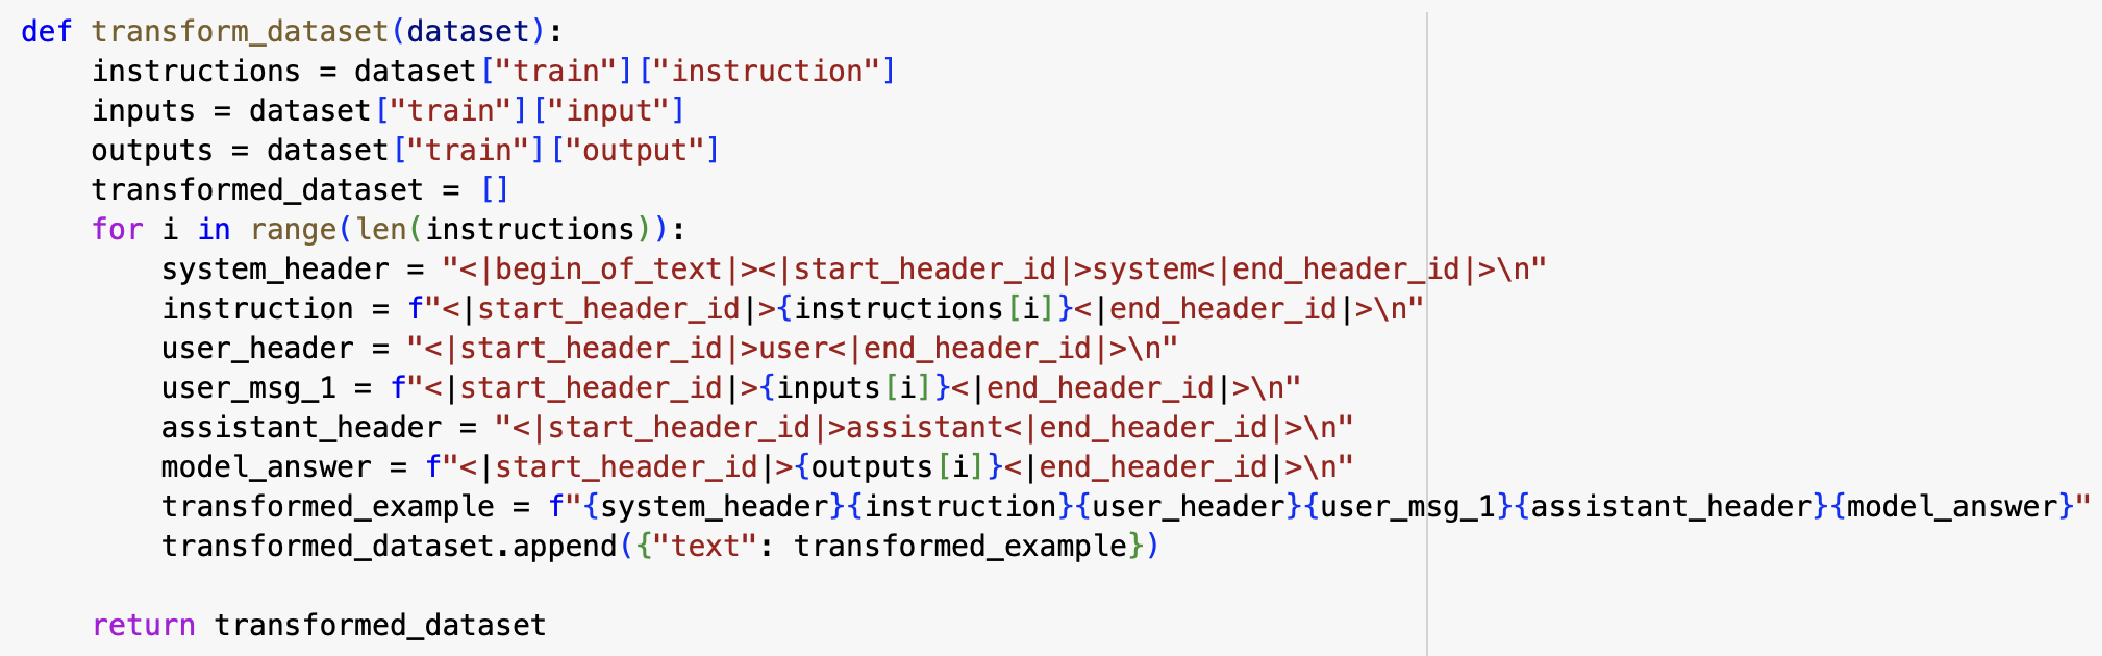
\includegraphics[width=14.5cm]{img/promptFormat.pdf}
        \caption{Funzione per costruire il \textit{prompt} adeguato a \textit{Phi3-mini}}
    \end{figure}\newline
    %PROMPT FORMAT CODICE
    %perchè il prompt è importante
    L'ultimo passaggio prima di effetturare effettivamente il \gls{fine-tuning} è stato definire i parametri per l'allenamento, come ad esempio \textit{per\_device\_batch\_size}, \textit{optim}, \textit{learning\_rate}, \textit{max\_step}.
    In questo caso si è deciso di avere una grandezza di \textit{batch} pari a 16, ciò va a specificare il numero di esempi utilizzati per ogni iterazione del \textit{fine-tuning} del modello. 
    Rigurardo a \textit{optim}, l'ottimizzatore, si è deciso di utilizzare \textit{adamw\_torch} il quale è un algorimo di ottimizzazione che unisce i benefit dell'ottimizzatore \textit{Adam} con \textit{weight decay} (regolarizzazione) per prevenire l'\textit{overfitting}.
    La \textit{learning\_rate} invece è il tasso di apprendimento e determina quanto velocemente o lentamente un modello apprende. È un fattore di scalatura che regola quanto devono essere aggiornati i pesi del modello in risposta all'errore calcolato in ogni iterazione dell'addestramento. Per questo parametro è stato scelto $5\times10^-^5$ poichè dopo alcuni esperimenti è risultato essere il miglior valore di \textit{tradeoff} tra velocità e precisione.
    \begin{figure}[htp]
        \centering        
        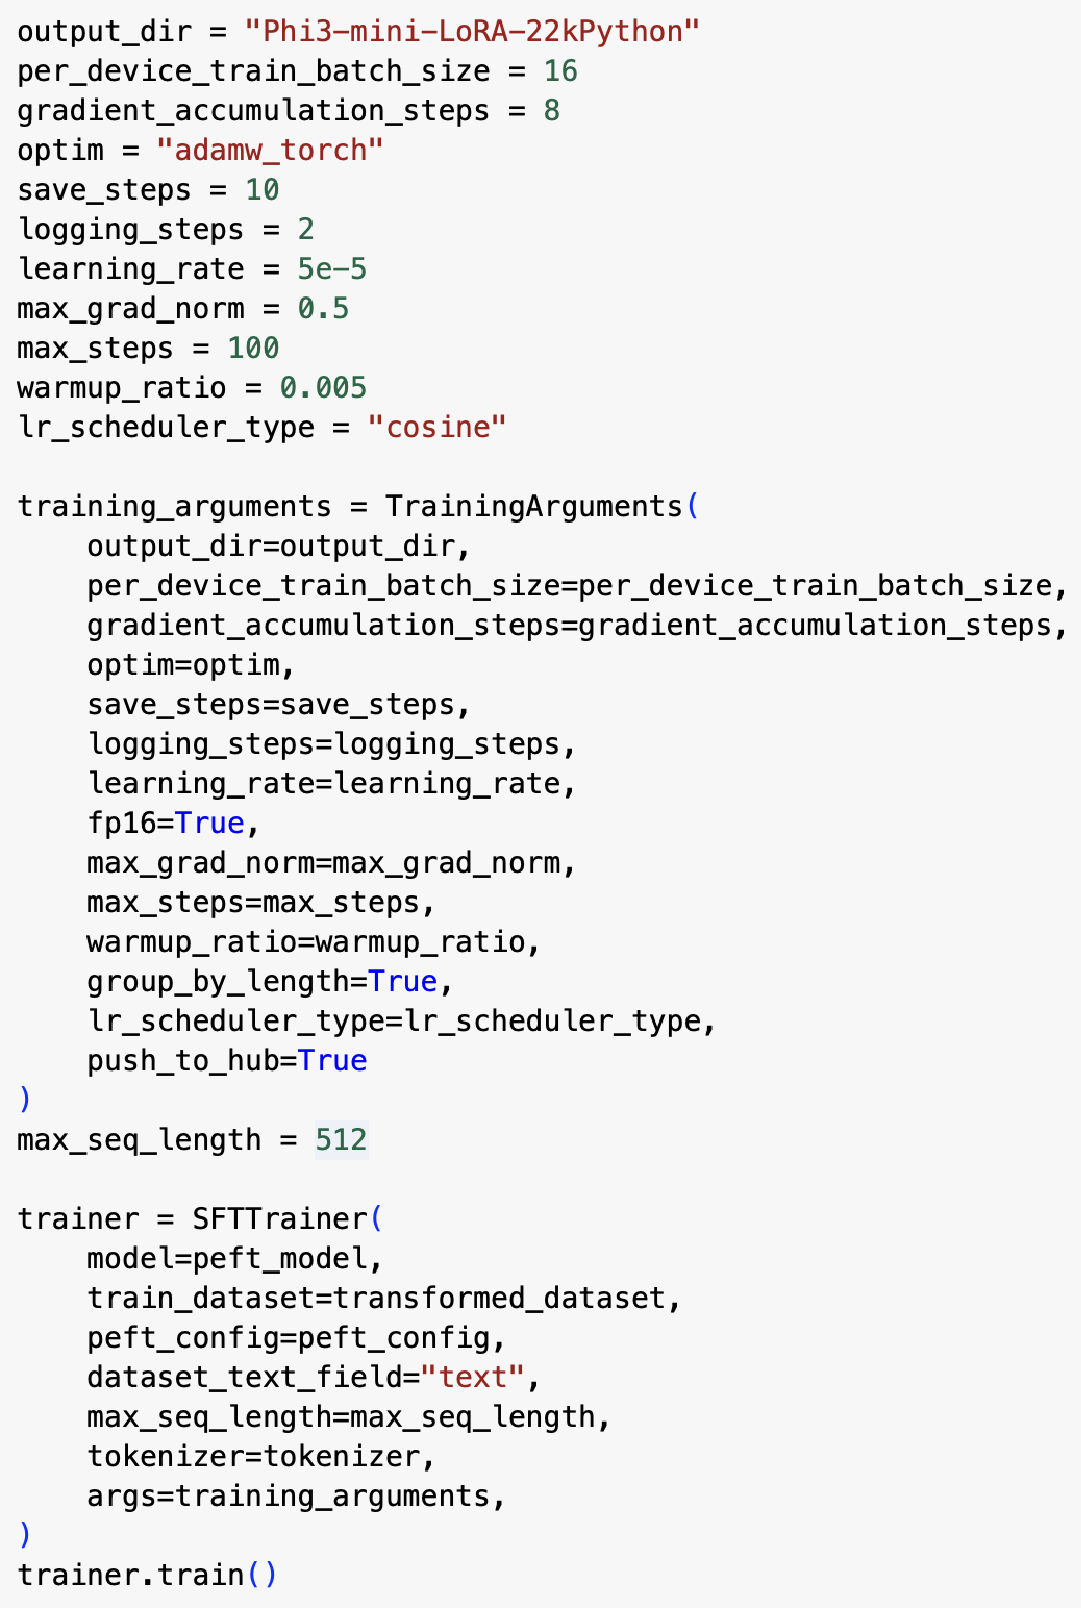
\includegraphics[width=12cm]{img/training.pdf}
        \caption{Esempio di codice per l'addestramento}
    \end{figure}\newpage

    %spiega il training


    \subsection{\textit{Fine-tuning attraverso LLama.cpp}}
      Oltre all'utilizzo di \textit{Colab}, è stato successivamente eseguito il \gls{fine-tuning} attraverso \textit{LLama.cpp}. A differenza di \textit{Colab}, \textit{LLama.cpp} prevede una semplificazione del codice e consente di utilizzarlo senza limiti computazionali, salvo quelli imposti dalle proprie risorse hardware.
    \begin{lstlisting}[language=bash]
        llama.cpp\finetune.exe
            --model-base model.gguf
            --train-data trainer.txt
            --lora-out Lora.gguf
            --threads 14
            --batch 8
            --sample-start "<s>"
            --ctx 1024
            --use-checkpointing
            --checkpoint-out LoRAModelCheckpoint-ITERATION.gguf
            --adam-iter 8192
            --adam-alpha 0.001
            --lora-r 16
            --lora-alpha 16
            --fill-with-next-samples
            --epoch 3
            --separate-with-eos
    \end{lstlisting}
    
    %fine tuning con LLamacpp -> comando e quanto ci ha messo 
        \subsection{Ottimizzazioni del fine-tuning}
        \subsubsection{Mixture of LoRA Experts}
        % estrai info da paper
        Il framework \textit{Mixture of} \gls{lora} \textit{Expert} rappresenta un metodo di \gls{fine-tuning} che si basa sull'utilizzo di \gls{lora}. Introdotta per la prima volta da Wu et al. \cite{article:Wu2024MixtureOL}, questa tecnica mira a risolvere i problemi legati alla riduzione delle capacità generative dei modelli affinati tramite \gls{lora}.
        Nel contesto di un modello \textit{Mixture of} \gls{lora} \textit{Expert} nell'apprendimento automatico, una funzione di gating viene utilizzata per assegnare dinamicamente diversi input a diversi "esperti" (tipicamente sub-modelli o reti neurali) all'interno del modello complessivo come visibile in figura 4.7. La funzione di gating:\\
        \centerline{$ \sigma(W\times x + b)$,} determina il contributo o il peso di ciascun esperto per un dato input, decidendo efficacemente quale esperto o combinazione di esperti debba essere responsabile delle predizioni per quell'input.\\
        \begin{figure}[htp]
            \centering        
            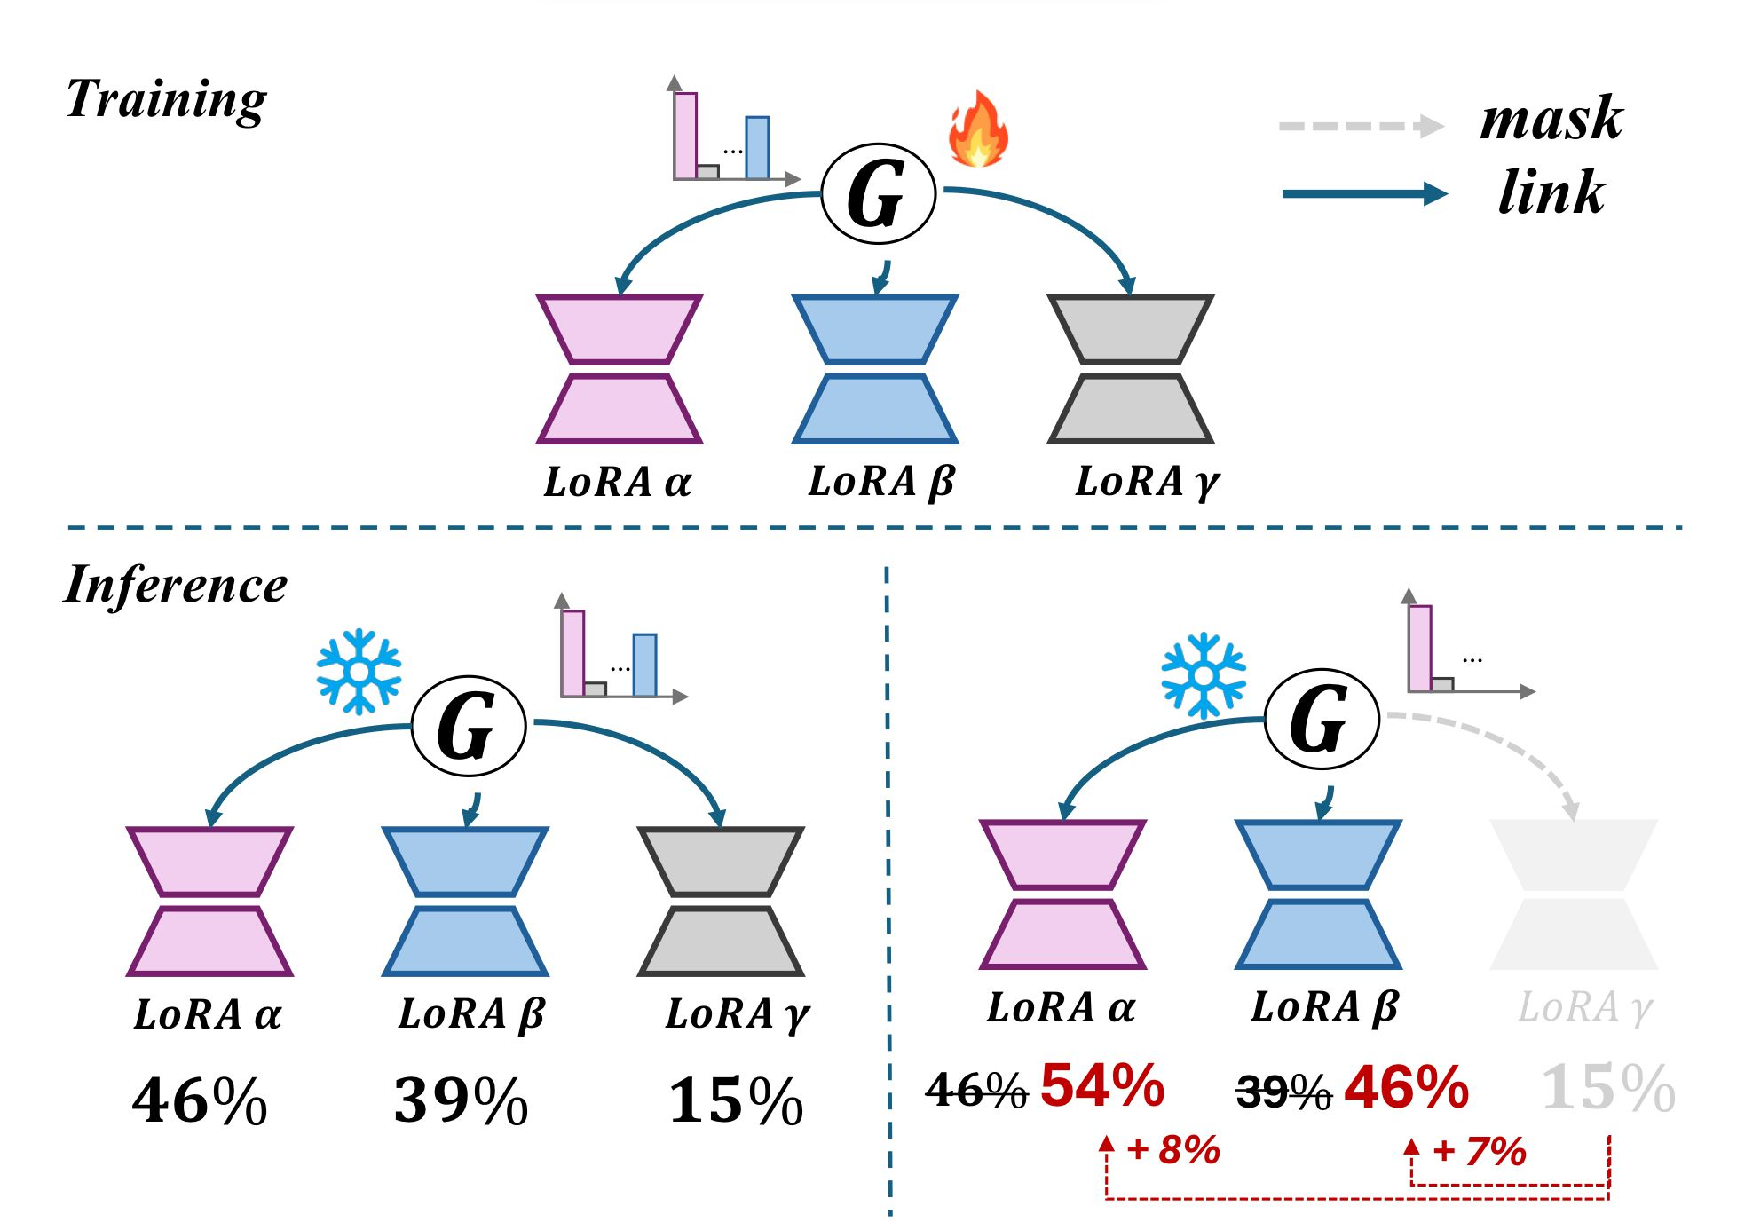
\includegraphics[width=10cm]{img/MoE2.pdf}
            \caption{Assegnazione dinamica dei LoRA \textit{layer} in Mixture of LoRA Expert}
        \end{figure}
       \newpage\textit{Mixture of} \gls{lora} \textit{Expert} consente l'impiego di diversi livelli di \gls{lora}, trattando ciascun livello addestrato con \gls{lora} come un esperto distinto. Implementa inoltre un controllo gerarchico del peso attraverso una funzione di gating che viene appresa all'interno di ogni livello, mantenendo congelati tutti gli altri parametri. In questo modo, è possibile apprendere pesi di composizione adattati specificamente agli obiettivi di un determinato dominio.
        \begin{figure}[htp]
            \centering        
            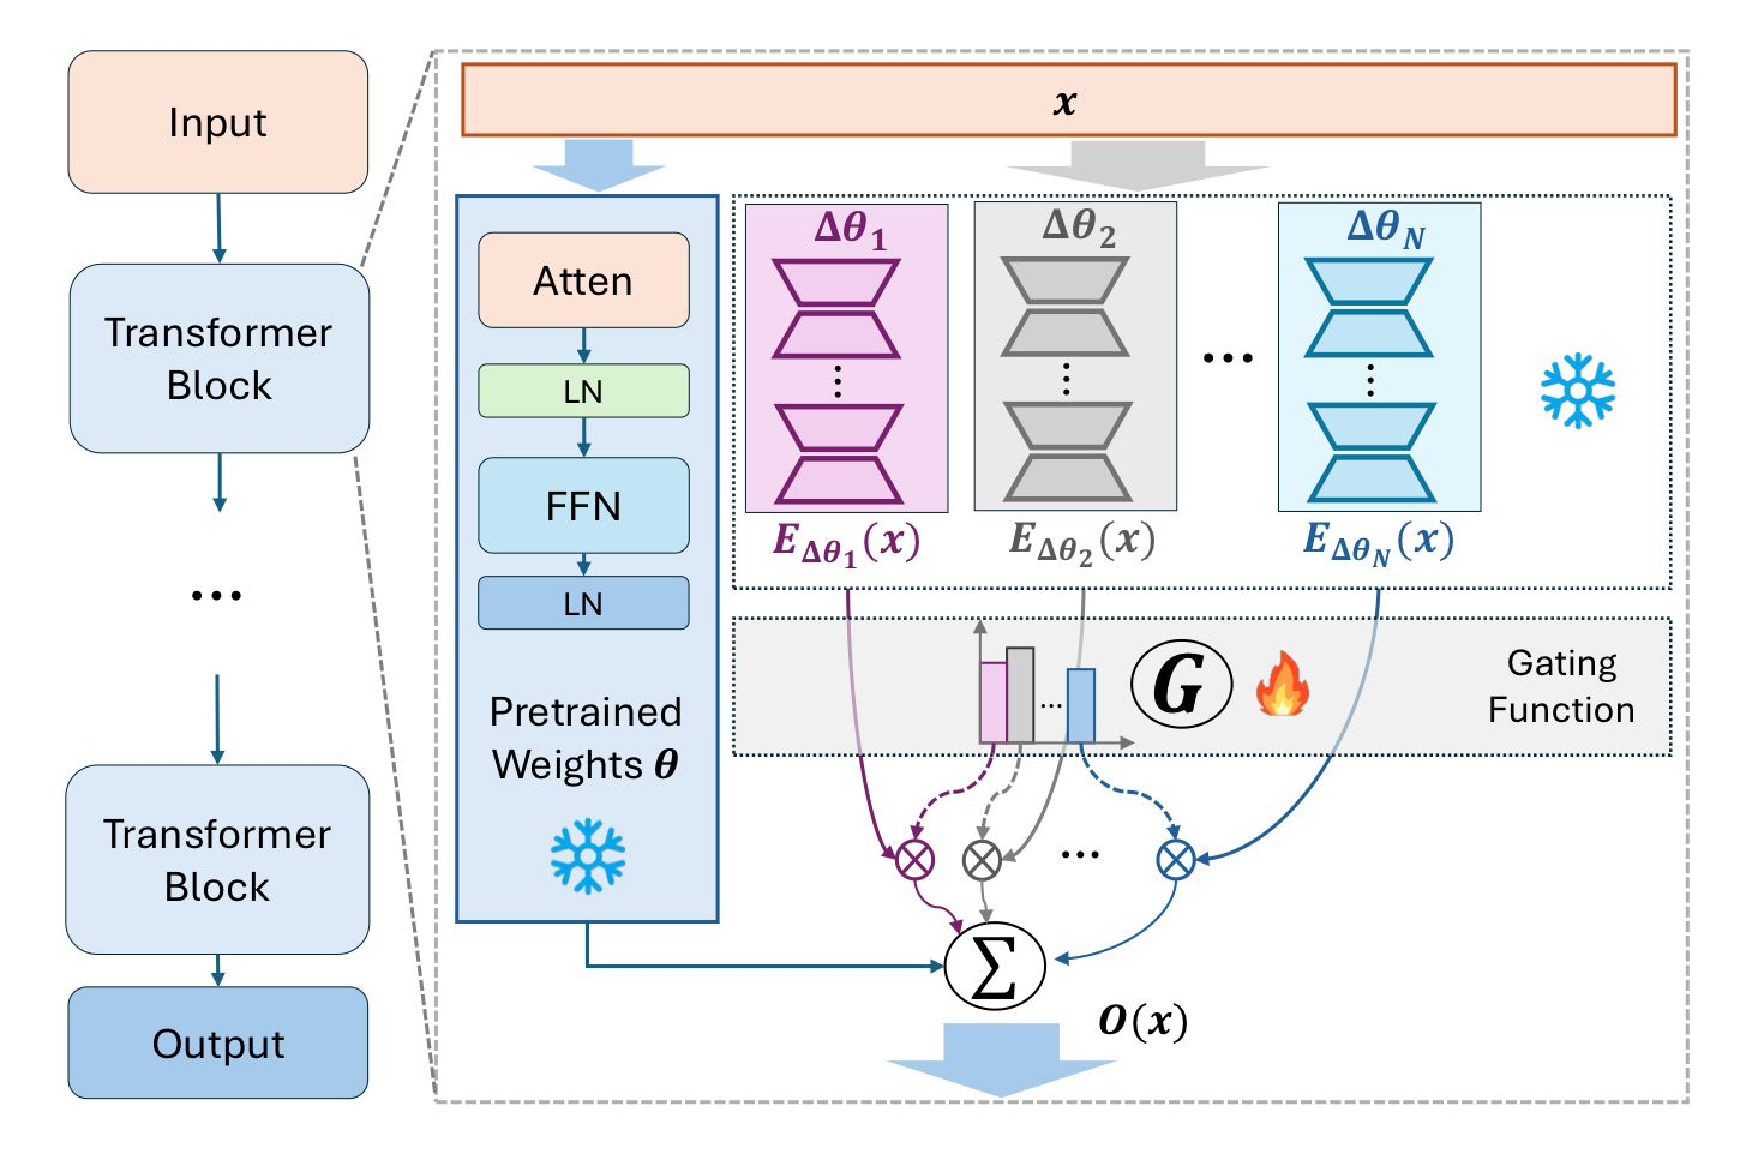
\includegraphics[width=10cm]{img/MoE1.pdf}
            \caption{Mixture of Expert all'intenro dell'architettura Transformer}
        \end{figure}

        
        I \textit{layer} quindi vengono integrati all'interno dell'architettura Transformer come visibile in figura 4.8.
        Come è visibile, l'idea di base di \gls{lora}, la quale consiste nel congelare i pesi pre-addestrati, continua ad essere presente, in parallelo, i \gls{lora} \textit{layer} dopo essere stati addestrati per specifiche \textit{task}, vengono sommati linearmente e il loro peso in questa somma viene determinato dalla funzione di gating.


        % MoLE -> 
        \subsubsection{AdaMoLE}
        \textit{Adaptive Mixture of} \gls{lora} \textit{Expert} è un metodo il quale utilizza \textit{Mixture of} \gls{lora} \textit{Expert} e una soglia di rilevanza, quest’ultima permette l’attivazione dei vari esperti solo se la loro percentuale di congruenza rispetto al contesto supera la soglia stessa.
        Questo procedimento permette una selezione dinamica degli   esperti attivando quindi solamente gli esperti che sono più appropriati rispetto al contesto (\textit{context-responsive}), ciò porta ad una migliore adattabilità e performance più elevate.
        \begin{figure}[htp]
            \centering        
            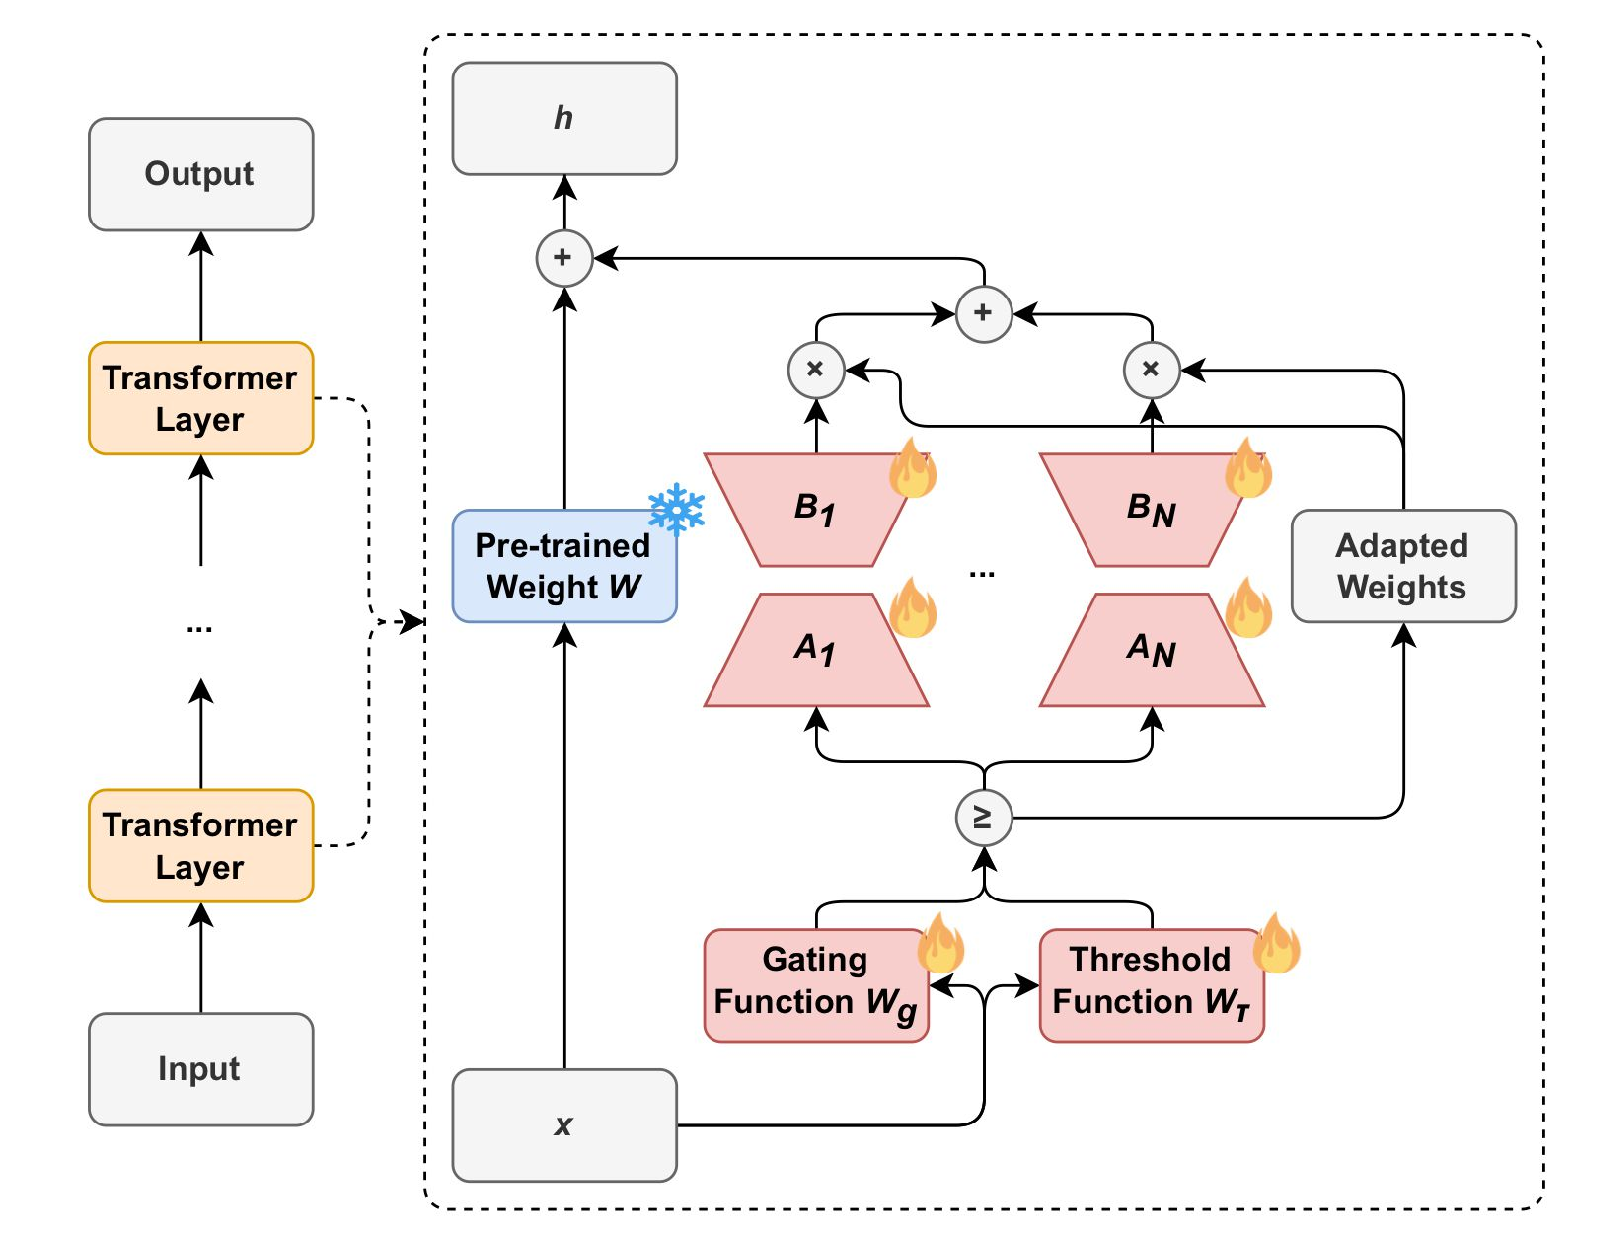
\includegraphics[width=10cm]{img/AdaMOle.pdf}
            \caption{Strutture AdaMoLE nell'architettura Transformer}
        \end{figure}\newline
        In figura 4.9 è possibile notare la scelta dei vari esperti, la soglia e la gating function sono parte fondamentale di tutto il processo.
        Successivamente, dopo aver valutato gli esperti, i loro output vengono combinati per produrre la risposta finale del sistema. Questo può essere fatto attraverso pesi adattivi che tengono conto della rilevanza di ciascun esperto per l'input corrente.\\
        Ricordando che la distribuzione dei pesi ai vari esperti è $\rho_i$, con:\\
        \centerline{$\rho_i = SoftMax(W_gx)_i$,}
        e il risultato della somma degli output è:\\
        \centerline{$y=\sum_{i=1}^N \frac{\operatorname{TopK}\left(p_i\right)}{\sum_{i^{\prime}=1}^N \operatorname{TopK}\left(p_{i^{\prime}}\right)} \cdot E_i(x)$,}
        mentre la decisione di utilizzare un determinato esperto deriva da:\\ \centerline{$\rho_i \geq \tau$, con $\tau$ come soglia}\newline
        È possibile intuire che è di massima importanza scegliere una soglia $\tau$ adeguata, infatti $\rho_i \geq \tau$, questo perchè scegliendo $\tau$ troppo elevata si potrebbero escludere tutti i layer e quindi avere un risultato che non è frutto del modello con \gls{fine-tuning}.
        D'altra parte se la soglia fosse troppo bassa questo potrebbe includere layer non rilevanti per il contesto.
        Per mitigare queste possibili problematiche si utilizza $\tau = \frac{1}{N}$, da ciò deriva che $\sum_{i=1}^N\rho_i \geq N\tau = 1$ contraddicendo il fatto che $\rho_i$ debba essere uguale a 1.
        L'output quindi derivante da AdaMoLE è:\\
        \centerline{$y=\sum_{i=1}^N \frac{\mathds{1}\left(p_i \geq \tau\right) \cdot p_i}{\sum_{i^{\prime}=1}^N \mathds{1}\left(p_{i^{\prime}} \geq \tau\right) \cdot p_{i^{\prime}}} \cdot E_i(x)$,}
        Con $\mathds{1}$ uguale a 1 se la condizione $\rho_i \geq \tau$ è vera, 0 altrimenti.

        % AdaMoLE
    \subsection{Quantizzazione}
    La quantizzazione di un \gls{llm} è una tecnica utilizzata per ridurre le dimensioni del modello e aumentare l'efficienza computazionale senza una significativa perdita di accuratezza. Questa tecnica converte i parametri del modello (tipicamente rappresentati come numeri in virgola mobile a 32-bit floating point) in una rappresentazione con meno bit, ad esempio con interi a 8-bit o a 16-bit ed in alcuni casi estremizzando a 4-bit o 2-bit.
    La quantizzazione è una tecnica ormai necessaria per permettere l'utilizzo degli \gls{llm} su qualsiasi dispositivo poichè hanno raggiunto dimensioni computazionalmente proibitive per molti dei dispositivi mobile.
    Durante il secondo macroperiodo vi è stata la possibilità di affrontare l'argomento quantizzazione, in paricolare si è approfondita la quantizzazione asimmetrica e simmetrica.
    Entrambe le metodologie mirano a comprimere i modelli per renderli più efficienti in termini di memoria e velocità di calcolo, ma differiscono nel modo in cui i valori vengono mappati nello spazio quantizzato.
    \begin{figure}[htp]
    \centering
    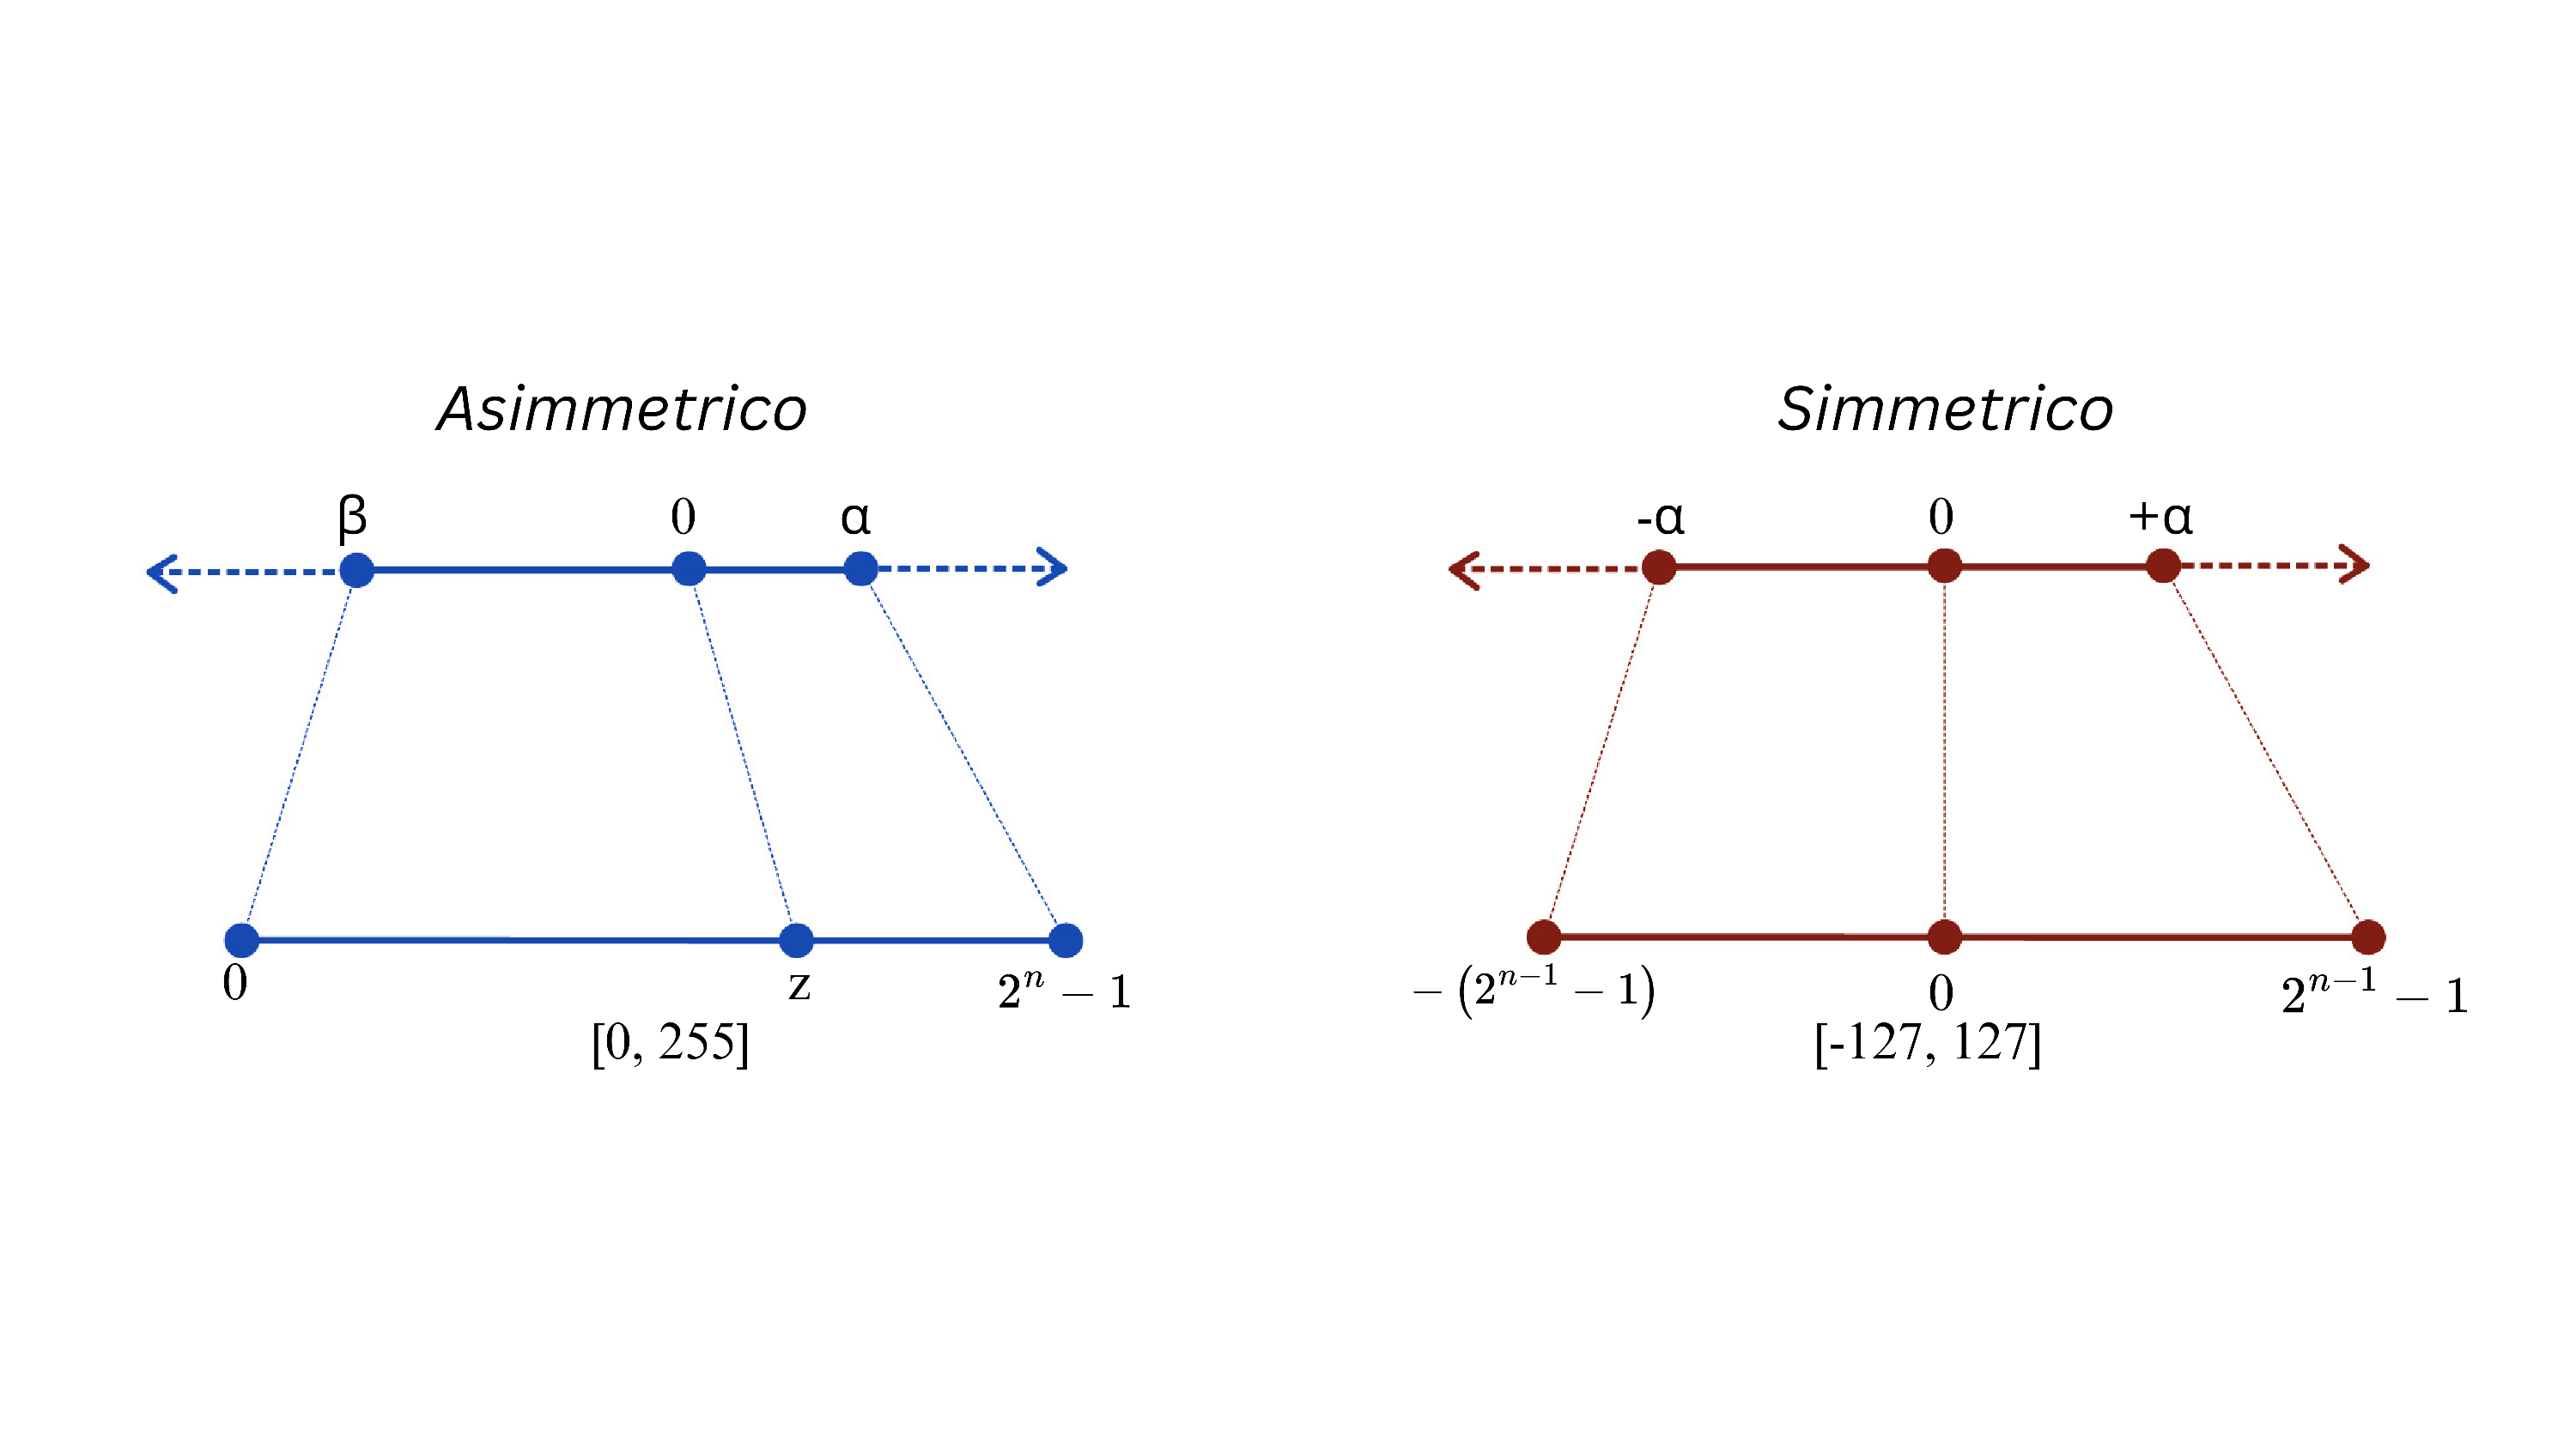
\includegraphics[width=13cm]{img/AsymmetricSymmetric.pdf}
    \caption{Differenza tra tecnica asimmetrica e simmetrica}
    \end{figure}
    \\
    Quantizzazione Asimmetrica:
    \begin{itemize}
        \item \textbf{Scala Non Uniforme}: Nella quantizzazione asimmetrica, i valori del modello vengono mappati in uno spazio quantizzato che non è centrato attorno allo zero. L'intervallo dei valori positivi e negativi è solitamente diverso e dipende da $\alpha$ e $\beta$
        \item \textbf{Range di Quantizzazione}: Viene definito un fattore di scala $s$ diverso per i valori positivi e negativi, o un valore di offset $z$ che permette di gestire l'intervallo in modo più flessibile.
        \item \textbf{Flessibilità Maggiore}: Permette una rappresentazione più precisa per distribuzioni di valori che non sono simmetriche attorno allo zero.
    \end{itemize}
    Per ottenere la quantizzazione asimmetrica, $x_q$ del numero $x_f$ si utilizzano le seguenti formule:
    
    \centerline{$x_q=\operatorname{clamp}\left(\left\lfloor\frac{x_f}{s}\right\rfloor+z ; 0 ; 2^n-1\right) \quad s=\frac{\alpha-\beta}{2^n-1} \quad z=\left\lfloor-1 \times \frac{\beta}{s}\right\rfloor$}
    
    In caso si volesse riconvertire al numero originario il numero quantizzato attraverso la tecnica asimmetrica la formula è la seguente:\\
    \centerline{$x_f = s(x_q-z)$.}
    Quantizzazione Simmetrica:
    \begin{itemize}
        \item \textbf{Scala Uniforme}: Nella quantizzazione simmetrica, i valori del modello vengono mappati in uno spazio quantizzato che è centrato attorno allo 0, sostanzialmente lo 0 quantizzato rimane 0. Ciò significa che l'intervallo dei valori positivi e negativi è uguale.
        \item \textbf{Range di Quantizzazione}: Viene definito un unico fattore di scala $s$ che determina come i valori in virgola mobile vengono convertiti in valori interi. Questo fattore di scala è uguale per i valori positivi e negativi.
        \item  \textbf{Semplicità di Implementazione}: La simmetria attorno allo zero rende più semplici i calcoli e diminuisce l'hardware necessario per la quantizzazione.
    \end{itemize}
    Per ricavare quindi il numero quantizzato $x_q$ è necessario applicare le seguenti formule:
    \centerline{$x_q=\operatorname{clamp}\left(\left\lfloor\frac{x_f}{s}\right\rfloor ;-\left(2^{n-1}-1\right) ; 2^{n-1}-1\right) \quad s=\frac{|\alpha|}{2^{n-1}-1}$}
    Nel caso in cui invece si volesse riconvertire al numero originario il numero quantizzato attraverso la tecnica simmetrica la formula è la seguente:\\
    \centerline{$x_f = sx_q$.}


    % cos'è 
    % a cosa serve
    % cosa si è utilizzato -> quantizzazione di un modello preaddestrato vedi Colab
    \subsubsection{Sviluppo}
    Per la quantizzazione, si è proceduto direttamente quantizzando Phi3-mini. Come visibile in figura 4.4, il modello, che ha subito il fine-tuning, è stato precedentemente quantizzato da 32-bit floating point a 8-bit interi. Questo è stato possibile attraverso il seguente frammento di codice:
    
    \begin{figure}[htp]
    \centering
    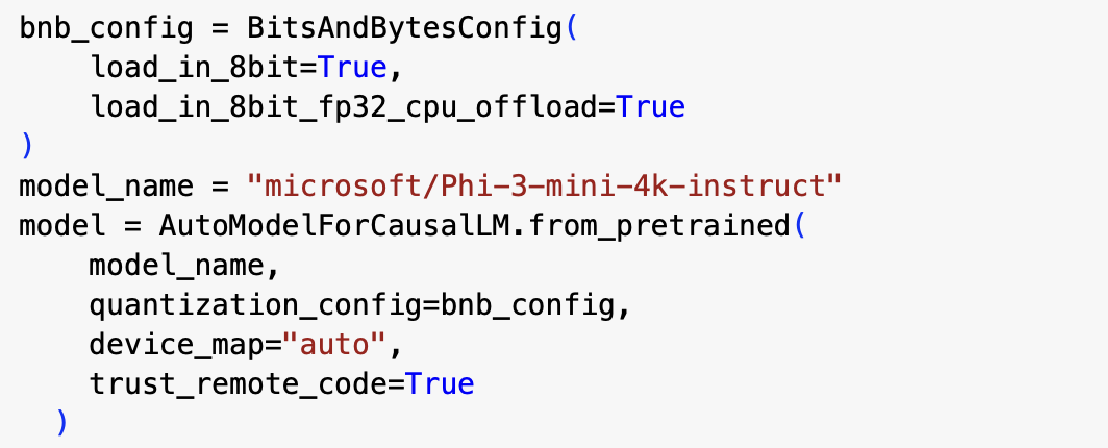
\includegraphics[width=10cm]{img/bitsAndBytes.pdf}
    \caption{Errore relativo asimmetrico suddiviso nei diversi bit di quantizzazione}
    \end{figure}
    In particolare, si è utilizzato il plugin BitsAndBytesConfig, che permette di quantizzare a 8-bit o a 4-bit qualsiasi modello.
    La quantizzazione ha quindi reso possibile una maggiore velocità per l'inferenza e inoltre anche un consumo ridotto delle risorse a disposizione.

    \subsubsection{Test errore di quantizzazione}
     È noto che scalando 32-bit in un numero di bit minore vi sarà sicuramente una perdita, anche minima, di informazione. In seguito è possibile visionare errore relativo in percentuale che deriva dalla quantizzazione.\\
     \centerline{$errore\_relativo = \frac{|x - x_q|}{\DeclarePairedDelimiter{|x|}}$, con $x$ valore a 32-bit, e $x_q$, valore quantizzato,}
     In figura 4.11 e 4.12 è possibile visualizzare in percentuale l'errore relativo asimmetrico e simmetrico rispetto a 1000 valori.
    \begin{figure}[!h]
        \centering        
        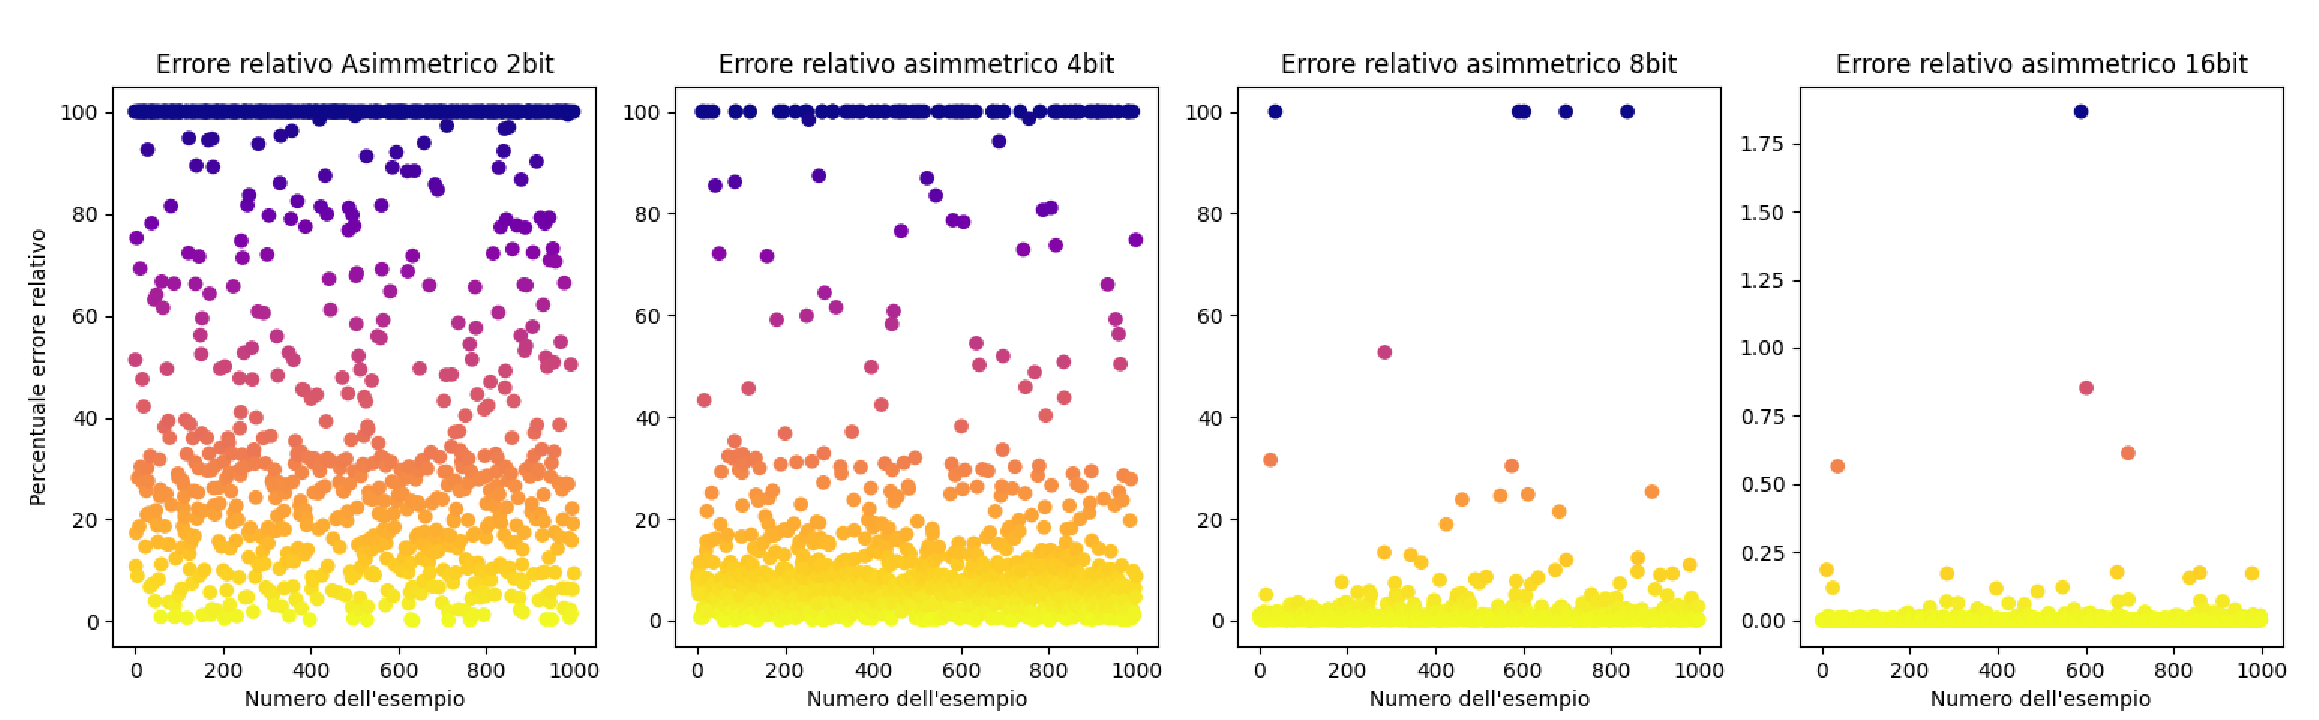
\includegraphics[width=14.5cm]{img/totA.pdf}
        \caption{Errore relativo asimmetrico suddiviso nei diversi bit di quantizzazione}
    \end{figure}\newline
    \begin{figure}[!h]
        \centering        
        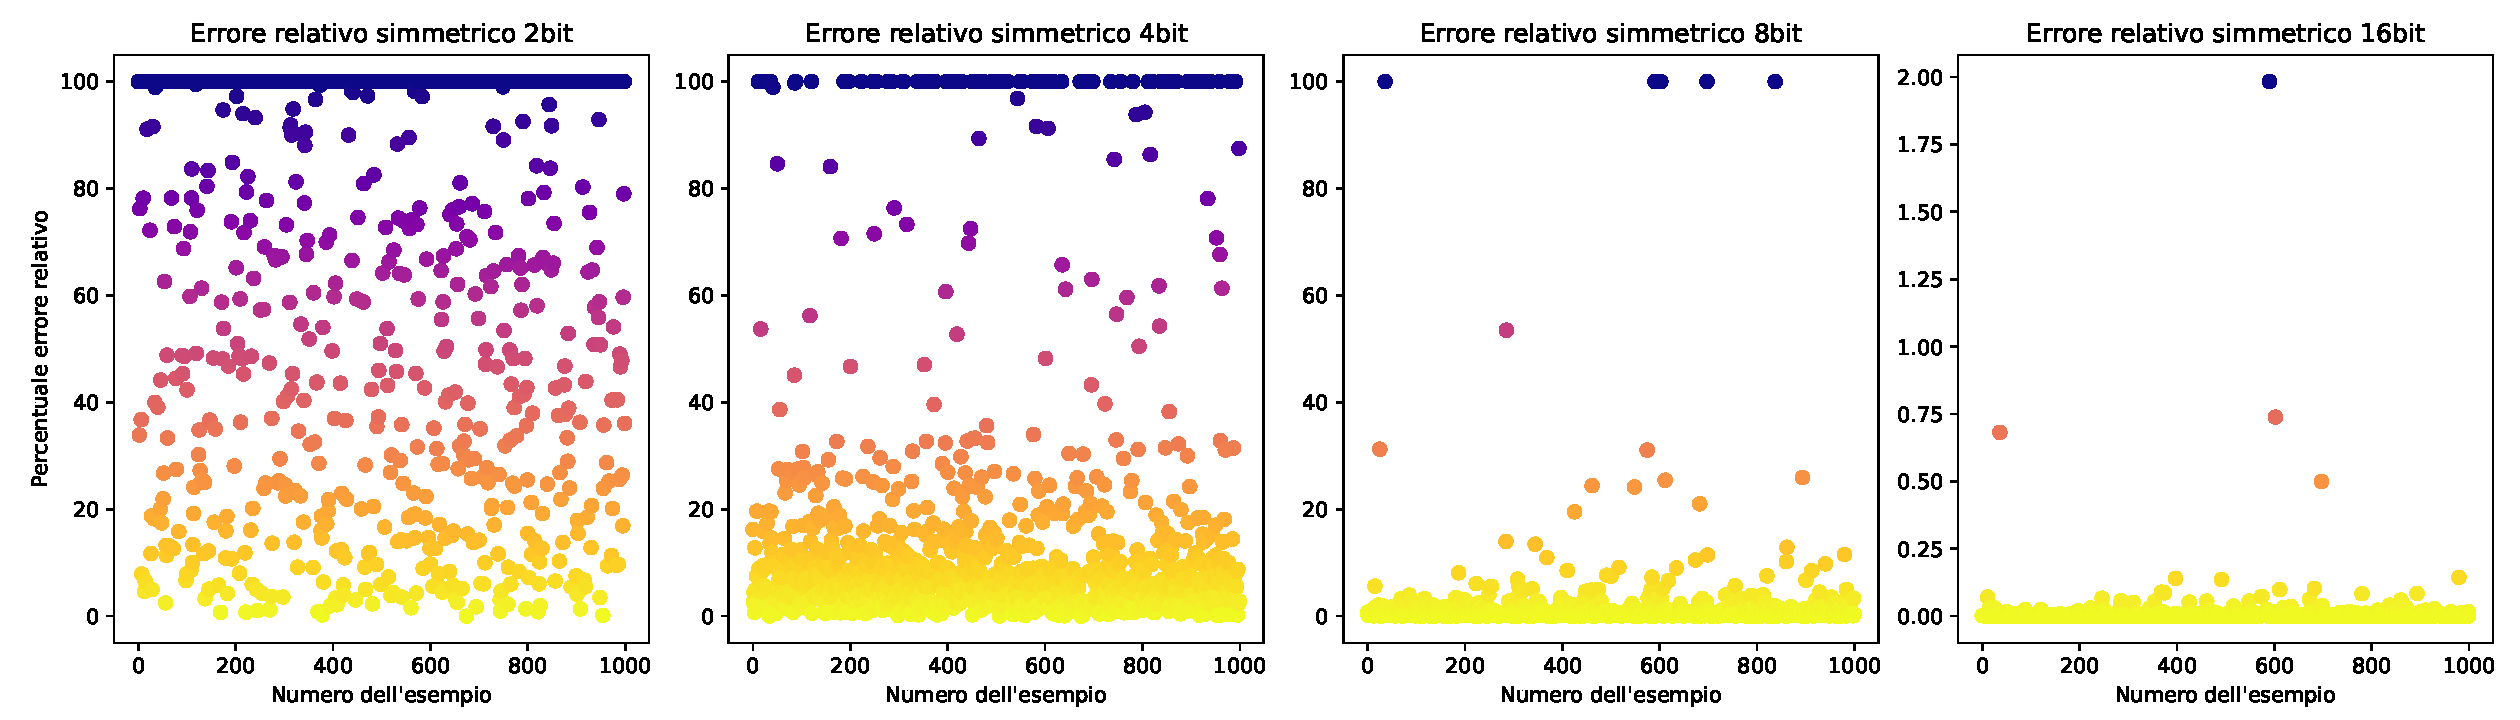
\includegraphics[width=14.5cm]{img/totS.pdf}
        \caption{Errore relativo simmetrico suddiviso nei diversi bit di quantizzazione}
    \end{figure}    
    \newline
    % test su perdita di dati della quantizzazione

    
\section{Resoconto finale}
    \subsection{Prodotti ottenuti}
        %loss function di modelli addestrati con colab e llamacpp
    \subsection{Risultati ottenuti}
        % bene o male, pro e contro del PROGETTO e di come è stato affrontato
        % bene perchè si sono notati risultati
        
        % male perchè costoso 
    \subsection{Conclusione}
    

\newpage